\documentclass[11pt]{article}
\usepackage[margin=1in]{geometry}
\usepackage{graphicx}
\usepackage{booktabs}
\usepackage[hypertexnames=false]{hyperref}
\usepackage{amsmath}
\usepackage{float}
\usepackage{enumitem}
\usepackage{xcolor}

\title{DM2026 Assignment 3: Human Activity Recognition}
\author{Yu-Shun Liu \\ Student ID: 413551030}
\date{}

\begin{document}
\maketitle

\noindent\textbf{GitHub Repository:} \url{https://github.com/RaisoLiu/DM2026-Assignment-3}

\noindent\textbf{Kaggle Public Score:} 0.8106, public leaderboard, submitted 2026-05-05.

\noindent\textbf{Selected Submission File:} \texttt{submissions/submission\_lgbm\_leaves63\_calibrated.csv}

\noindent\textbf{Selected Submission SHA-256:}
\begin{verbatim}
f78034a7e72d25ab4d52baebed585e130ad810e1f5cfae7469205008d5d5035e
\end{verbatim}

%==============================================================================
\section{How to Run the Code}
%==============================================================================

The implementation uses Python 3 and the packages listed in \texttt{requirements.txt}.
The Kaggle archive is downloaded with:

\begin{verbatim}
kaggle competitions download -c nycu-data-mining-assignment-3 -p data/raw --force
unzip -q -o data/raw/nycu-data-mining-assignment-3.zip -d data/raw
\end{verbatim}

The downloaded archive contains \texttt{train/train/User\_*} and
\texttt{test/test/User\_*}. I move the \texttt{User\_*} directories one level up
so the final layout is:

\begin{verbatim}
data/raw/train/User_001/*.csv ... data/raw/train/User_060/*.csv
data/raw/test/User_061/*.csv  ... data/raw/test/User_100/*.csv
data/raw/sample_submission.csv
\end{verbatim}

The final Kaggle CSV is reproduced by:

\begin{verbatim}
python scripts/make_boosting_submission.py \
  --results-csv artifacts/model_search_position_proba/results_position.csv \
  --model lgbm_leaves63 \
  --context position \
  --output submissions/submission_lgbm_leaves63_calibrated.csv \
  --seed 2026
\end{verbatim}

\texttt{make\_boosting\_submission.py} trains the explored LightGBM model on all
labeled windows, applies the OOF class calibration weights, and writes a
Kaggle-compatible \texttt{Id,Label} CSV aligned to \texttt{sample\_submission.csv}.
The earlier HGB baseline and feature-family ablations are reproduced by
\texttt{scripts/run\_experiment.py}.

%==============================================================================
\section{Preliminary Analysis and Design Motivation}
%==============================================================================

The training set contains 11,020 five-minute windows from 60 users. The test set
contains 6,849 windows from 40 disjoint users. Each file has 300 one-second rows
with \texttt{mean\_x}, \texttt{mean\_y}, \texttt{mean\_z}, \texttt{std\_x},
\texttt{std\_y}, \texttt{std\_z}, \texttt{index}, and \texttt{file\_id}; training
files also contain one repeated file-level \texttt{label}.

The task is strongly imbalanced (Figure~\ref{fig:class-dist}). Since the official
metric is macro-F1, accuracy is not sufficient. A model can achieve high accuracy
by mostly predicting labels 0 and 1, but it will lose macro-F1 on the minority
activities. I therefore use user-grouped cross-validation and class-balanced
training weights. Grouping by \texttt{User\_*} is important because the test users
are disjoint from training users; random window splits would leak user-specific
orientation, calibration, and wearing-style information.

\begin{figure}[H]
\centering
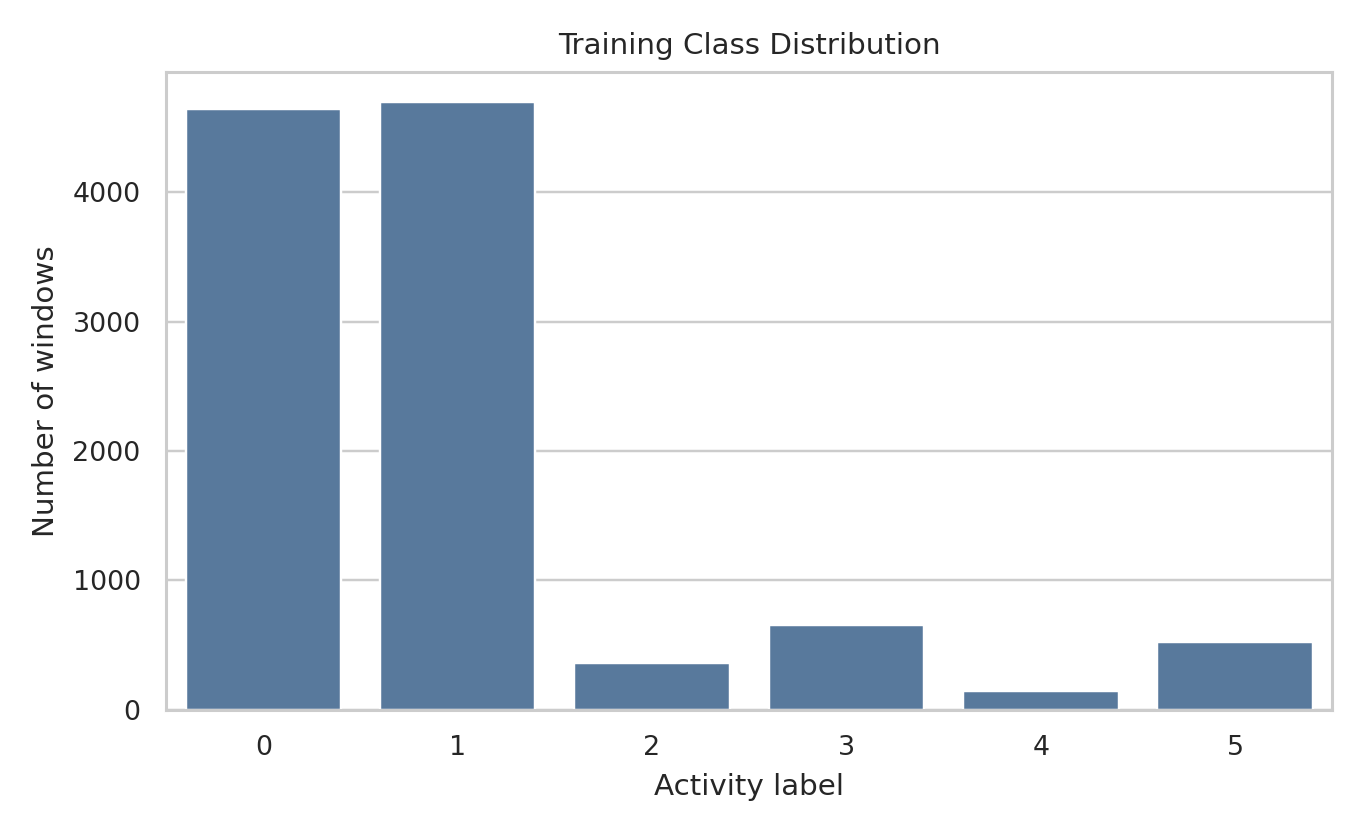
\includegraphics[width=0.72\textwidth]{figures/class_distribution.png}
\caption{Training class distribution. Labels 0 and 1 account for 84.7\% of
training windows, while label 4 has only 142 examples.\label{fig:class-dist}}
\end{figure}

\begin{table}[H]
\centering
\caption{Training class counts and fractions\label{tab:class-counts}}
\begin{tabular}{rcc}
\toprule
Label & Count & Fraction \\
\midrule
0 & 4,643 & 42.13\% \\
1 & 4,695 & 42.60\% \\
2 & 358 & 3.25\% \\
3 & 656 & 5.95\% \\
4 & 142 & 1.29\% \\
5 & 526 & 4.77\% \\
\bottomrule
\end{tabular}
\end{table}

The accelerometer retains the gravity component. This makes vector magnitude and
orientation informative: activities can differ by both motion intensity and wrist
posture. The preliminary feature check showed that the average mean-vector
magnitude is close to 1g (\texttt{mean\_vm\_mean} median 0.997), while dynamic
variability (\texttt{std\_vm\_mean}) ranges widely. This motivated a file-level
feature representation combining static gravity-aware features and temporal
variability features.

%==============================================================================
\section{Preprocessing and Feature Engineering}
%==============================================================================

Each CSV is sorted by \texttt{index}, interpolated within the six signal channels,
and converted into one feature vector. I do not train on individual seconds as
independent samples because the label belongs to the whole five-minute window.

The base feature table has 399 engineered features per window. The final
LightGBM submission adds six user-sequence position features, giving 405
features:

\begin{table}[H]
\centering
\caption{Feature families used by the selected LightGBM model\label{tab:features}}
\begin{tabular}{p{0.28\textwidth}p{0.60\textwidth}}
\toprule
Feature family & Purpose \\
\midrule
Global channel statistics & Quantiles, RMS, range, skewness, and kurtosis. \\
Gravity/magnitude & Vector magnitude, deviation from 1g, dynamic/static ratio. \\
Temporal derivatives & First-difference volatility, energy, and zero-crossings. \\
Segment/rolling & Five one-minute segments plus 5/15/30-second rolling variability. \\
Frequency & FFT power, dominant frequency, entropy, centroid, and band ratios. \\
Cross-axis/orientation & Axis-normalized orientation, correlations, and covariance. \\
User sequence position & Normalized order, reverse order, edge distance, sine/cosine phase, and sequence length. \\
\bottomrule
\end{tabular}
\end{table}

The most important preprocessing choice is keeping the prediction unit at the
file level. Feature extraction and final submission both align by \texttt{file\_id};
the submission is merged back to \texttt{sample\_submission.csv} by \texttt{Id}.

%==============================================================================
\section{Label Alignment and Temporal Dependency Modeling}
%==============================================================================

Each 300-row file corresponds to exactly one activity label. The pipeline uses
the following alignment:

\begin{enumerate}[leftmargin=*]
    \item Read one CSV file and sort rows by \texttt{index}.
    \item Infer the single \texttt{file\_id} and, for training, the single label.
    \item Extract one window-level feature vector from all 300 seconds.
    \item Train and validate on one row per file.
    \item Predict one label per test \texttt{file\_id}.
    \item Merge predictions to \texttt{sample\_submission.csv} in the original
    \texttt{Id} order.
\end{enumerate}

Temporal dependencies are represented through deterministic sequence summaries.
First differences capture second-to-second motion changes. Segment statistics
preserve coarse order over the five-minute interval. Rolling statistics capture
local bursts or sustained variability. FFT summaries capture periodicity at the
available 1 Hz resolution. This design is simpler and more reproducible than a
deep sequence model, while still respecting the temporal nature of the data.

%==============================================================================
\section{Core Model and Validation Strategy}
%==============================================================================

The final submitted model is \texttt{LGBMClassifier} with \texttt{num\_leaves=63},
900 estimators, class-balanced sample weights, and the 405-feature
position-augmented window representation. I kept the HGB pipeline as the
baseline for feature-family ablations because it is deterministic, fast, and
easy to stress-test. The validation protocol is 5-fold grouped cross-validation
by user with seed 2026. Grouped CV is deliberately more conservative than a
random window split because the public/private test set contains unseen users.

The selected prediction applies out-of-fold class-bias calibration. I first
collect OOF predicted probabilities from grouped CV, then tune one multiplicative
decision weight per class to maximize macro-F1 on the OOF predictions. This does
not retrain the model or use test labels; it only adjusts the decision rule to
match the official macro-F1 objective.

\begin{table}[H]
\centering
\caption{Class decision weights selected from OOF macro-F1 calibration\label{tab:calibration}}
\begin{tabular}{rc}
\toprule
Class & Weight \\
\midrule
0 & 0.41647 \\
1 & 0.45553 \\
2 & 5.85992 \\
3 & 0.89605 \\
4 & 1.31184 \\
5 & 0.76524 \\
\bottomrule
\end{tabular}
\end{table}

For the final LightGBM model, calibration increased grouped OOF macro-F1 from
0.72509 to 0.74771. The main gain was improved recall for label 2, a rare class
that otherwise tends to be absorbed into labels 1 and 3.

\begin{table}[H]
\centering
\caption{Grouped CV and public leaderboard model search summary\label{tab:cv}}
\begin{tabular}{lcc}
\toprule
Model / decision rule & OOF Macro-F1 & Public score \\
\midrule
HGB baseline, calibrated & 0.73823 & 0.7922 \\
XGBoost position model, calibrated & \textbf{0.74977} & 0.7933 \\
LightGBM leaves63 position model, calibrated & 0.74771 & \textbf{0.8106} \\
\bottomrule
\end{tabular}
\end{table}

\begin{table}[H]
\centering
\caption{Calibrated 5-fold grouped CV classification report\label{tab:class-report}}
\begin{tabular}{rccc}
\toprule
Label & Precision & Recall & F1 \\
\midrule
0 & 0.97537 & 0.98083 & 0.97809 \\
1 & 0.90484 & 0.91949 & 0.91211 \\
2 & 0.28536 & 0.32123 & 0.30223 \\
3 & 0.68714 & 0.73323 & 0.70944 \\
4 & 0.92537 & 0.87324 & 0.89855 \\
5 & 0.86881 & 0.56654 & 0.68585 \\
\midrule
Macro avg & 0.77448 & 0.73243 & \textbf{0.74771} \\
\bottomrule
\end{tabular}
\end{table}

\begin{figure}[H]
\centering
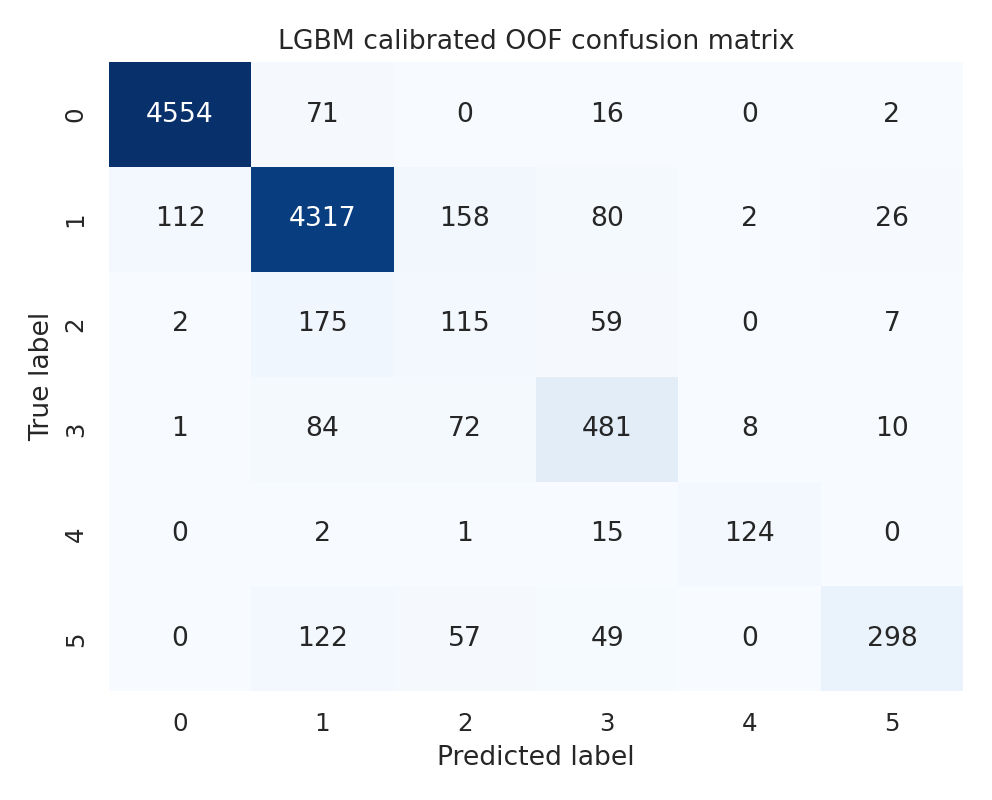
\includegraphics[width=0.68\textwidth]{figures/calibrated_confusion_matrix.png}
\caption{Calibrated LightGBM 5-fold OOF confusion matrix. The dominant residual error is
label 2 being confused with labels 1 and 3.\label{fig:confusion}}
\end{figure}

%==============================================================================
\section{Ablation Study}
%==============================================================================

I used the same fast HGB configuration for feature-family ablations. Each
ablation removes one feature family and reruns 5-fold grouped CV.

\begin{table}[H]
\centering
\caption{Feature-family ablation with grouped CV\label{tab:ablation}}
\begin{tabular}{lcc}
\toprule
Design & Macro-F1 & Delta from full \\
\midrule
Full feature set & 0.72921 & 0.00000 \\
Remove gravity/magnitude & 0.71548 & -0.01373 \\
Remove temporal derivatives & 0.72808 & -0.00113 \\
Remove segment/rolling & 0.73131 & +0.00210 \\
Remove frequency & 0.72923 & +0.00002 \\
Remove orientation/cross-axis & 0.73168 & +0.00246 \\
\bottomrule
\end{tabular}
\end{table}

\begin{figure}[H]
\centering
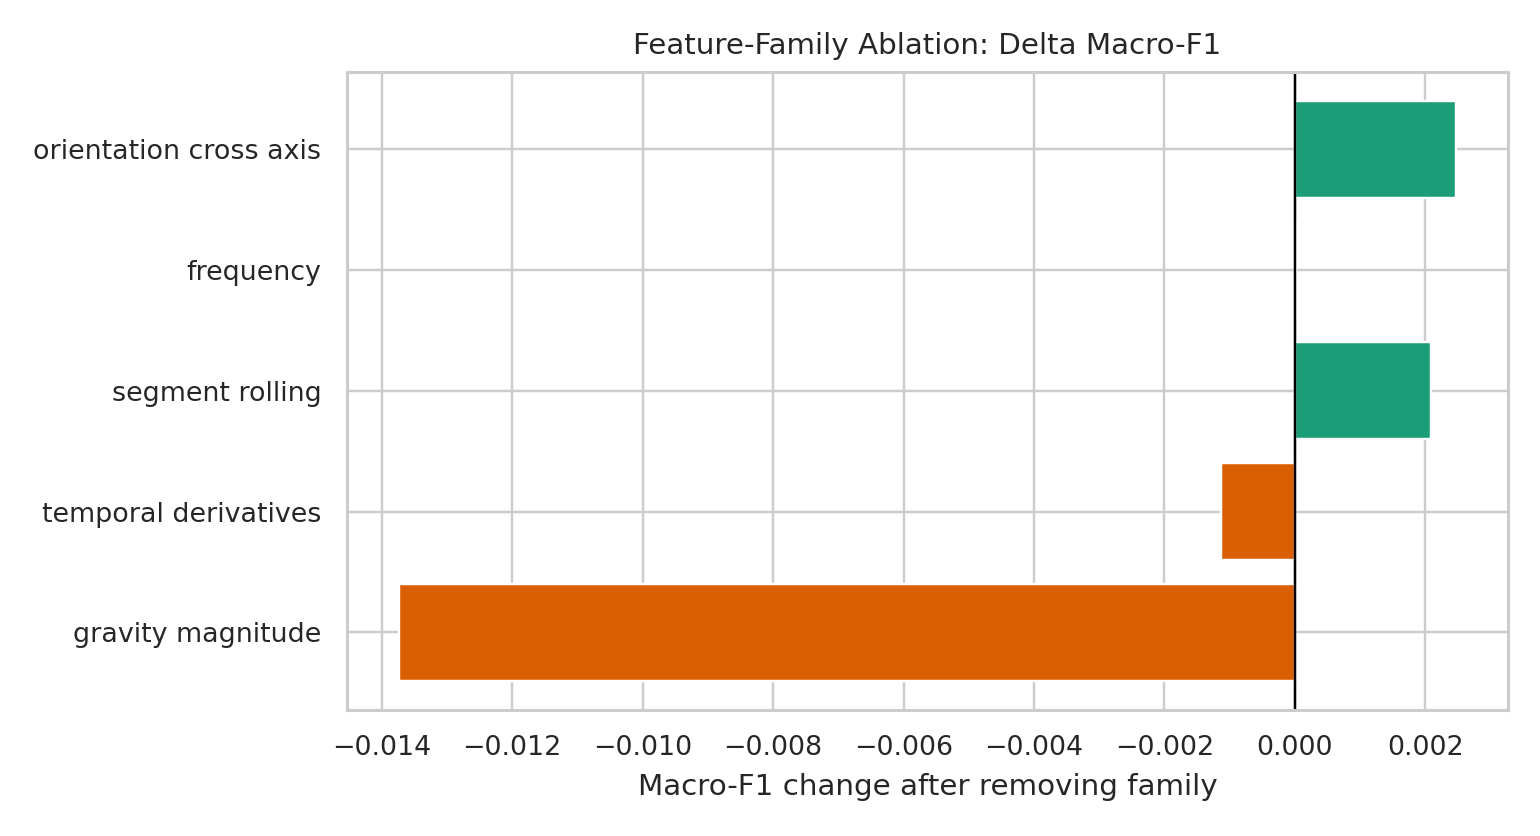
\includegraphics[width=0.82\textwidth]{figures/feature_ablation_delta.png}
\caption{Macro-F1 change after removing each feature family. Gravity/magnitude
features are the clearest positive contributor.\label{fig:ablation}}
\end{figure}

The largest loss comes from removing gravity/magnitude features, confirming that
the retained gravity component is useful. Removing segment/rolling or
orientation/cross-axis features slightly improves the uncalibrated HGB score in
this split, suggesting mild fold-specific noise. I therefore used the ablation
as evidence for the feature representation rather than as a final model
selector. The final LightGBM submission keeps the complete engineered feature
set and adds only compact user-position features.

I also tested a full 450-iteration HGB. It reached calibrated OOF macro-F1
0.74751, but its calibrated test predictions assigned label 2 to 15.56\% of test
windows, compared with only 3.25\% in the training set. The final LightGBM
submission has a more plausible test prior: label 2 is 2.76\%, label 4 is
1.26\%, and labels 0/1 remain dominant. It also produced the best observed public
leaderboard score, 0.8106 (Figure~\ref{fig:submission-dist}).

\begin{figure}[H]
\centering
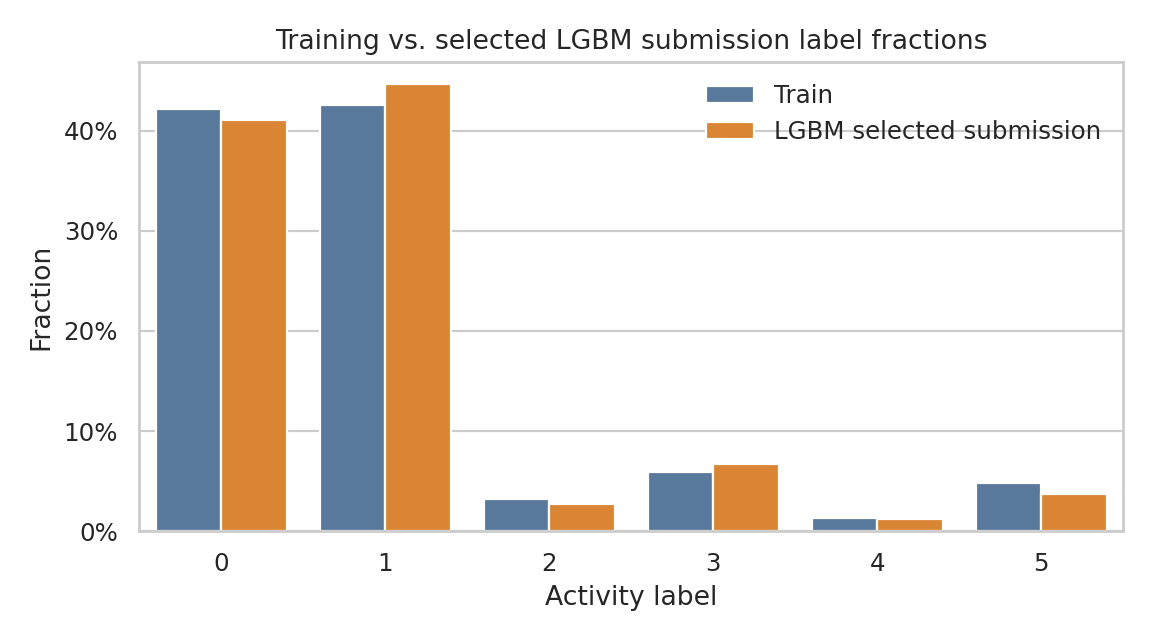
\includegraphics[width=0.76\textwidth]{figures/submission_distribution.png}
\caption{Training label fractions compared with the final LightGBM submission's
predicted label fractions. The selected submission keeps rare-class priors close
to the training distribution while improving public leaderboard score.\label{fig:submission-dist}}
\end{figure}

%==============================================================================
\section{Residual Risks and Next Steps}
%==============================================================================

The main residual error is label 2. Even after calibration, label 2 F1 is only
0.30223 in grouped OOF validation, with many examples confused as labels 1 or 3.
This is the highest-value
target for future improvement because macro-F1 weights every class equally. The
next experiments I would prioritize are:

\begin{itemize}[leftmargin=*]
    \item stronger label-2 focused calibration constrained by plausible test priors;
    \item user-level bootstrap stability checks for calibration weights;
    \item a small sequence model or 1D convolution benchmark using the same
    grouped validation protocol;
    \item ensembling only models whose test label priors remain plausible.
\end{itemize}

The final selected CSV was submitted to Kaggle and scored 0.8106 on the public
leaderboard. The submitted file is format-checked: 6,849 rows, columns exactly
\texttt{Id,Label}, label range 0--5, no missing labels, and ID order matching
\texttt{sample\_submission.csv}. I keep all submitted files and scores in
\texttt{SUBMISSION\_LOG.md}; the competition allows three submissions per day.

\end{document}
